\documentclass[12pt, a4paper]{article}
\usepackage[utf8]{inputenc}
\usepackage{hyperref}
\usepackage{graphicx}
\usepackage{listings}
\usepackage{xcolor}
\usepackage{float}
\usepackage{caption}
\usepackage{subcaption}

\definecolor{codegreen}{rgb}{0,0.6,0}
\definecolor{codegray}{rgb}{0.5,0.5,0.5}
\definecolor{codepurple}{rgb}{0.58,0,0.82}
\definecolor{backcolour}{rgb}{0.95,0.95,0.92}

\lstdefinestyle{mystyle}{
    backgroundcolor=\color{backcolour},   
    commentstyle=\color{codegreen},
    keywordstyle=\color{magenta},
    numberstyle=\tiny\color{codegray},
    stringstyle=\color{codepurple},
    basicstyle=\ttfamily\footnotesize,
    breakatwhitespace=false,         
    breaklines=true,                 
    captionpos=b,                    
    keepspaces=true,                 
    numbers=left,                    
    numbersep=5pt,                  
    showspaces=false,                
    showstringspaces=false,
    showtabs=false,                  
    tabsize=2
}

\lstset{style=mystyle}

\hypersetup{
    colorlinks=true,
    linkcolor=black,
    urlcolor=cyan,
}

\graphicspath{{img/}}


\title{\textbf{Elaborato di Intelligenza Artificiale} \\ Implementazione di una Simulazione con Modelli di Reti Neurali Utilizzando l'Ambiente di Sviluppo Python}
\author{Soldà Matteo --- 1226319}
\date{\today}

\begin{document}

\begin{figure}
    \centering
    \includegraphics[width=0.60\textwidth]{Logo_Università_Padova}
\end{figure}

\maketitle

\newpage
\begin{abstract}
Nel presente elaborato verrà implementata una simulazione tramite modelli di reti neurali utilizzando l'ambiente di sviluppo Python.\\
La simulazione si baserà sul database \textit{MNIST}, riguardante il riconoscimento di numeri manoscritti, fornitoci durante la terza esercitazione pratica.\\
Dopo aver introdotto i vari tipi di rete e i loro risultati tramite un breve report, si cercherà rispondere a tre domande essenziali: definire le cifre più difficili da riconoscere, quantificare la variazione di accuratezza dovuta all'inserimento di rumore nel \textit{training pattern} e la variazione dell'accuratezza di riconoscimento sul \textit{testing pattern} riducendo drasticamente le dimensioni del \textit{training pattern}.    
\end{abstract}

\newpage
\tableofcontents

\newpage
\section{Introduzione}
In questo elaborato si prenderà in considerazione uno dei problemi più famosi che vengono sottoposti alle intelligenze artificiali: il riconoscimento di numeri manoscritti.
La simulazione chè verrà presentata si baserà sul dataset \href{http://yann.lecun.com/exdb/mnist/}{\textit{MNIST}}, il quale contiene 70.000 immagini, con relative etichette, di cifre comprese tra 0 e 9 scritte a mano.\\
Per risolvere il problema sopra descritto, utilizzeremo due Percettroni Multi-Strato: la variante classica e quella convoluzionale.\\
Inizialmente verranno create diverse versioni con diversi numeri di strati nascosti e diversi numeri di neuroni per strato, si procederà poi con la creazione di altrettanti percettroni convoluzionali per poi concludere con il confronto tra le varie reti create per capire quali siano le più performanti. A seguire si risponderà ai tre quesiti sopra citati.
Per lo sviluppo di questa simulazione, sono stati creati due notebook su \href{https://colab.research.google.com/?utm_source=scs-index}{Google Colaboratory}, accessibili in visualizzazione per chiunque visiti i link sottostanti:
\begin{itemize}
    \item \href{https://colab.research.google.com/drive/1e4vY_9wn6-ugL5NivZc0RBluGdfWqTUM?usp=sharing}{NoteBook per il confronto approfondito tra MLP}
    \item \href{https://colab.research.google.com/drive/1v2dkWKelr-q5CTpsDUDqp55PUqiId64F?usp=sharing}{NoteBook per la risoluzione dei quesiti}
\end{itemize}

\newpage
\section{Analisi e Report --- Performance delle Reti}
Prima di addentrarsi nei quesiti, si proverà ad analizzare varie MLP per capire quali possano essere le più performanti per il riconoscimento dei numeri.\\
\subsection{Inizializzazione delle MLP --- Versione Classica}
Come prima cosa, sono state create 10 MLP classiche utilizzando la libreria \href{https://scikit-learn.org/stable/modules/generated/sklearn.neural_network.MLPClassifier.html#sklearn.neural_network.MLPClassifier}{\textit{sklearn.neural\_network}}, sotto meglio descritte:
\begin{itemize}
    \item \textbf{MLP2HL500}: MLP composta da 2 strati nascosti, ognuno dei quali da 500 neuroni;
    \item \textbf{MLP3HL500}: MLP composta da 3 strati nascosti, ognuno dei quali da 500 neuroni;
    \item \textbf{MLP5HL500}: MLP composta da 5 strati nascosti, ognuno dei quali da 500 neuroni;
    \item \textbf{MLP2HL100}: MLP composta da 2 strati nascosti, ognuno dei quali da 100 neuroni;
    \item \textbf{MLP5HL1000}: MLP composta da 5 strati nascosti, ognuno dei quali da 1000 neuroni;
    \item \textbf{MLP10HL150}: MLP composta da 10 strati nascosti, ognuno dei quali da 150 neuroni; 
    \item \textbf{MLP2HL250\_500}: MLP composta da 2 strati nascosti, contenenti rispettivamente 250 e 500 neuroni; 
    \item \textbf{MLP3HL250\_500\_1000}: MLP composta da 3 strati nascosti, contenenti rispettivamente 250, 500 e 1000 neuroni; 
    \item \textbf{MLP3HL1000\_500\_250}: MLP composta da 3 strati nascosti, contenenti rispettivamente 1000, 500 e 250 neuroni; 
    \item \textbf{MLP5HL100\_250\_500\_500\_500}: MLP composta da 5 strati nascosti, di cui i primi 2 strati contenenti rispettivamente 100 e 250 neuroni, mentre gli ultimi 3 saranno formati da 500 neuroni 
\end{itemize}
Tutte queste varianti utilizzano una funzione di attivazione "\href{https://it.wikipedia.org/wiki/Rettificatore_(reti_neurali)}{\textit{RELU}}", un risolutore basato su di un ottimizzatore \textit{gradient-based} denominato "\href{https://arxiv.org/abs/1412.6980}{\textit{adam}}" e un \textit{learning rate} costante di valore \(0.001\). \\
Queste MLP sono state addestrate per un periodo di 5 cicli sul training set. Nessuna di queste è riuscita a convergere, per questo ci viene restituito un \textit{warning}. \\
Di seguito la curva di apprendimento delle varie reti messe a confronto, oltre all'accuratezza prevista:
\begin{figure}[H]
    \centering 
    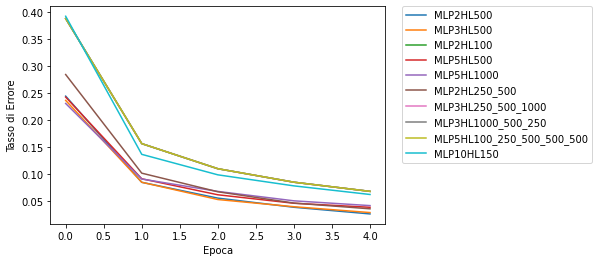
\includegraphics[width=\textwidth]{ConfrontoClassica.png}
\end{figure}
\begin{figure}[H]
    \centering
    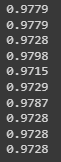
\includegraphics[width=0.2\textwidth]{AccuratezzaClassica.png}
\end{figure}

A seguire è stato effettuato anche un test delle reti su del rumore crescente nell'intervallo \([0.1 , 1.0]\), inserito tramite una funzione che aggiunge \href{https://it.wikipedia.org/wiki/Rumore_gaussiano}{rumore gaussiano}. Di seguito i risultati:
\begin{figure}[H]
    \centering
    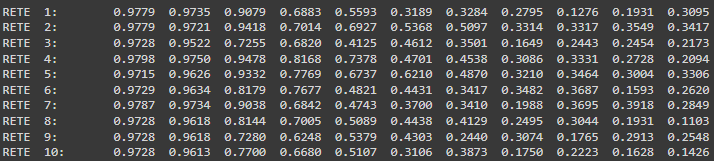
\includegraphics[width=\textwidth]{RisultatiRumoreClassica.png}
\end{figure}

\subsection{Inizializzazione delle MLP --- Versione Convoluzionale}
Si passa poi alle MLP convoluzionali, generate tramite il pacchetto \href{https://www.tensorflow.org/api_docs/python/tf/keras/Model}{\textit{tensorflow.keras}}. Di queste ne sono state create 6 diverse versioni, di seguito descritte:
\begin{itemize}
    \item \textbf{Conv2\_1428}: MLP composta da 2 strati convoluzionali rispettivamente con kernel \(3*3\) e \(4*4\), formata da 14 e 28 filtri, il tutto seguito da uno strato di pooling e infine da uno stato \textit{dense} di 10 unità;
    \item \textbf{Conv3\_142822}: MLP composta da 3 strati convoluzionali rispettivamente con kernel \(3*3\), \(4*4\) e \(4*4\), formata da 14, 28 e 22 filtri, il tutto seguito da uno strato di pooling e infine da uno stato \textit{dense} di 10 unità;
    \item \textbf{Conv10\_15}: MLP composta da 10 strati convoluzionali con kernel \(3*3\) formata da 15 filtri, il tutto seguito da uno strato di pooling e infine uno strato \textit{dense} di 10 unità; 
    \item \textbf{Conv5\_1428223050}: MLP composta da 5 strati convoluzionali rispettivamente con kernel \(3*3\), \(4*4\), \(5*5\), \(6*6\) e \(7*7\), formata da 14, 28, 22, 30 e 50 filtri, il tutto seguito da uno strato di pooling e infine da uno stato \textit{dense} di 10 unità;
    \item \textbf{Conv5\_1428405260}: MLP composta da 5 strati convoluzionali rispettivamente con kernel \(3*3\), \(4*4\), \(5*5\), \(6*6\) e \(7*7\), formata da 14, 28, 40, 52 e 60 filtri, il tutto seguito da uno strato di pooling e infine da uno stato \textit{dense} di 10 unità;
    \item \textbf{Conv1\_28}: MLP composta da un singolo strato convoluzionale formato da un kernel \(4*4\) da 28 filtri, seguito dallo strato di pooling e infine da uno strato \textit{dense} di 10 unità
\end{itemize}
Come descritto per la versione classica, anche la variante convoluzionale utilizza l'ottimizzatore "\href{https://arxiv.org/abs/1412.6980}{\textit{adam}}".\\
Analogamente alla versione classica, dato l'addestramento di 5 cicli, le reti non convergono. Di seguito la curva di apprendimento e l'accuratezza prevista delle reti:
\begin{figure}[H]
    \centering 
    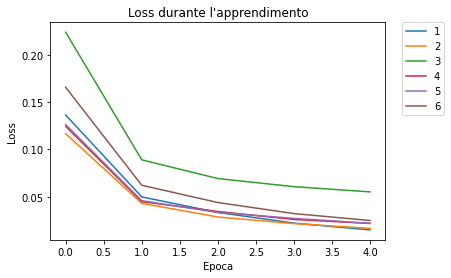
\includegraphics[width=.9\textwidth]{ConfrontoConvoluzionale.png}
\end{figure}
\begin{figure}[H]
    \centering
    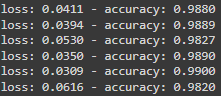
\includegraphics[width=0.6\textwidth]{AccuratezzaConvoluzionale.png}
\end{figure}

A seguire è stato effettuato anche un test su tutte le reti e su del rumore crescente per definire la resistenza al rumore. Di seguito i risultati:
\begin{figure}[H]
    \centering
    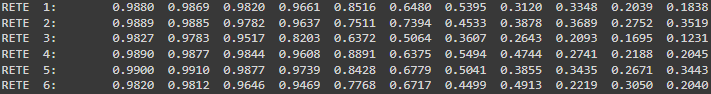
\includegraphics[width=\textwidth]{RisultatiRumoreConvoluzionale.png}
\end{figure}

\newpage
\subsection{Confronto tra Varianti}
Di seguito viene riportato il grafico che rappresenta il confronto tra tutte le MLP create:
\begin{figure}[H]
    \centering
    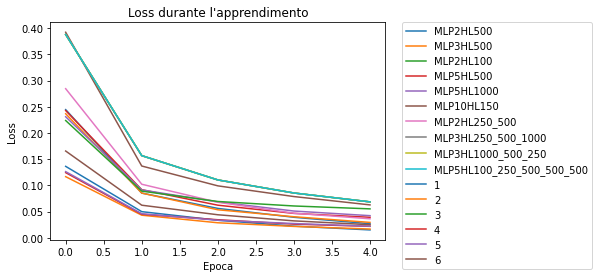
\includegraphics[width=\textwidth]{ConfrontoTotale.png}
\end{figure}
Analizzando i dati in nostro possesso, si può notare che, per le reti classiche, il numero ideale di strati nascosti deve essere compreso nell'intervallo \([2, 5]\) e che il numero di neuroni deve aggirarsi nell'intervallo \([250 , 500]\).
Di conseguenza, possiamo affermare che le reti migliori siano:
\begin{itemize}
    \item \textbf{MLP5HL500} \(>\) accuratezza \(0.9798\)
    \item \textbf{MLP2HL250\_500} \(>\) accuratezza \(0.9787\)
    \item \textbf{MLP2HL500 \& MLP3HL500} \(>\) accuratezza \(0.9779\)
\end{itemize} 

Per quanto riguarda invece le MLP convoluzionali, c'è da notare che globalmente surclassano l'accuratezza delle versioni classiche. Si sottolinea inoltre che le reti migliori sono risultate quelle con 5 strati convoluzionali e un numero di filtri e dimensione dei kernel relativamente crescenti. Di fatto le due migliori MLP risultano essere:
\begin{itemize}
    \item \textbf{Conv5\_1428405260} \(>\) accuratezza \(0.9900\)
    \item \textbf{Conv5\_1428223050} \(>\) accuratezza \(0.9890\)
\end{itemize}

\newpage
\section{Primo Quesito --- Numeri Difficili da Riconoscere}
\subsection{Visualizzazione di Pattern Erronei}
\paragraph{Warning:} da questo momento, e per la risoluzione di tutti i quesiti, si utilizzeranno MLP diverse (e possibilmente minori di numero) rispetto a quelle utilizzate nel report, ma che saranno addestrate nel primo e terzo quesito per un totale di 15 cicli. Di fatto verranno utilizzate sia versioni classiche che convoluzionali che rispecchiano l'affidabilità media per entrambe le classi, ossia \textit{MLP2HL500} e \textit{Conv2\_1428}, le quali sono state precedentemente descritte. \\\\ 
Per poter visualizzare al meglio le previsioni sbagliate, utilizzeremo tre liste di supporto:
\begin{itemize}
    \item sbagliate[]: contiene le "immagini" originali
    \item previsto[]: contiene il valore previsto dalla rete
    \item target[]: contiene il valore target associato al valore originario
\end{itemize}

Inizialmente verrà utilizzata una MLP classica, a seguire saranno mostrati anche i risultati della variante convoluzionale.
Di seguito i risultati:
\begin{figure}[H]
    \centering
    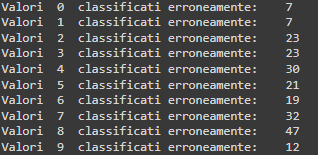
\includegraphics[width=0.50\textwidth]{ErrateClassica.png}
\end{figure}

Nella simulazione risulta che il numero che viene classificato più volte erroneamente è \(8\), che conta un numero di classificazioni errate di \(47\). A seguire il numero \(7\) e poi il \(4\). I numeri che invece vengono classificati in modo sbagliato poche volte sono \(0\), \(1\) e \(9\).\\
Di seguito alcuni esempi di numeri \(8\) che sono stati classificati in modo erroneo:

\begin{figure}[H]
    \centering
    \begin{subfigure}{.5\textwidth}
        \centering
        \caption{Numero Previsto: 0}
        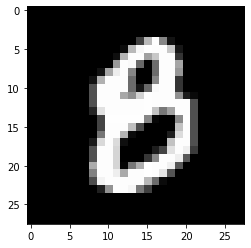
\includegraphics[width=0.50\textwidth]{otto1.png}
    \end{subfigure}% 
    \begin{subfigure}{.5\textwidth}
        \centering
        \caption{Numero Previsto: 4}
        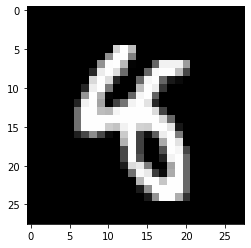
\includegraphics[width=0.50\textwidth]{otto2.png}
    \end{subfigure} 
\end{figure}

\begin{figure}[H]
    \begin{subfigure}{.5\textwidth}
        \centering
        \caption{Numero Previsto: 7}
        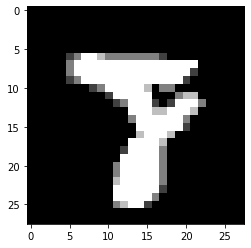
\includegraphics[width=0.50\textwidth]{otto3.png}
    \end{subfigure} %
    \begin{subfigure}{.5\textwidth}
        \centering
        \caption{Numero Previsto: 4}
        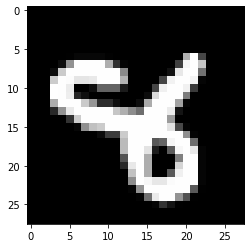
\includegraphics[width=0.50\textwidth]{otto4.png}
    \end{subfigure} 
\end{figure}

\begin{figure}[H]
    \centering
    \caption{Numero Previsto: 9}
    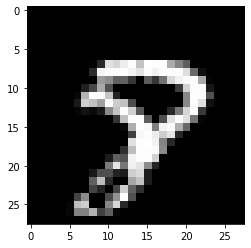
\includegraphics[width=0.25\textwidth]{otto5.png}
\end{figure} 

Per quanto riguarda la variante convoluzionale, si è utilizzato lo stesso metodo sopra descritto per l'estrazione dei valori classificati erroneamente e i risultati sono stati i seguenti:
\begin{figure}[H]
    \centering
    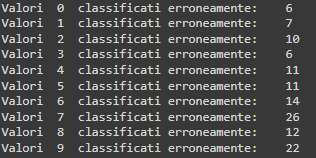
\includegraphics[width=0.50\textwidth]{ErrateConv.png}
\end{figure}
A differenza di quanto visto prima, i numeri che vengono mal classificati per la maggiore sono i \(9\) che contano un numero di classificazioni errate pari a 22. Da notare come globalmente il numero di classificazioni errate sia molto minore rispetto alla variante classica.\\
Di seguito alcuni esempi di \(9\) classificati erroneamente:

\begin{figure}[H]
    \begin{subfigure}{0.5\textwidth}
        \centering
        \caption{Numero Previsto: 5}
        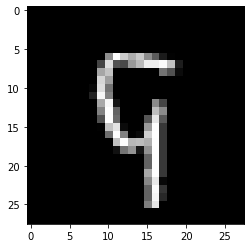
\includegraphics[width=0.50\textwidth]{nove1.png}
    \end{subfigure}
    \begin{subfigure}{0.5\textwidth}
        \centering
        \caption{Numero Previsto: 7}
        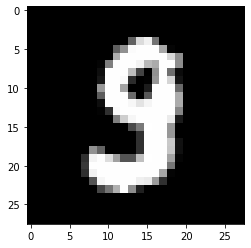
\includegraphics[width=0.50\textwidth]{nove2.png}
    \end{subfigure}
\end{figure}

\begin{figure}[H]
    \begin{subfigure}{0.5\textwidth}
        \centering
        \caption{Numero Previsto: 3}
        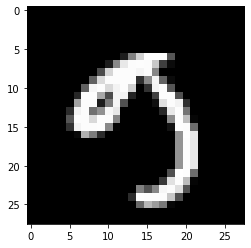
\includegraphics[width=0.50\textwidth]{nove3.png}
    \end{subfigure}
    \begin{subfigure}{0.5\textwidth}
        \centering
        \caption{Numero Previsto: 1}
        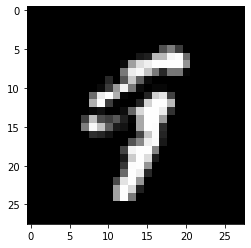
\includegraphics[width=0.50\textwidth]{nove4.png}
    \end{subfigure}
\end{figure}
\begin{figure}[H]
    \centering
    \caption{Numero Previsto: 1}
    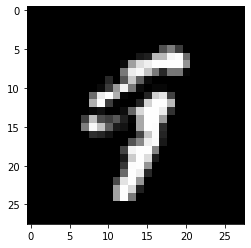
\includegraphics[width=0.25\textwidth]{nove5.png}
\end{figure}

\subsection{Aggiunta di Rumore in Pattern Corretti}
Per procedere con il quesito, prima di aggiungere del rumore, creiamo due nuove liste che conterranno le immagini e i target delle immagini che la rete ha classificato correttamente.\\
Il test è stato eseguito su rumori crescenti. La rete sarà considerata "affidabile" sino a quando il rateo di \textit{true positive} sarà maggiore del \(75\%\).\\
Per quanto riguarda la variante classica, la variazione dell'accuratezza risulta essere:
\begin{figure}[H]
    \centering
    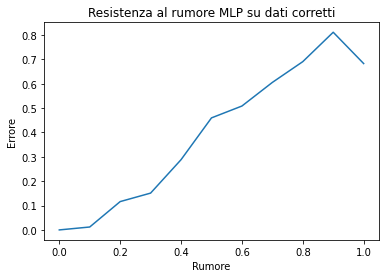
\includegraphics[width=0.50\textwidth]{TPClassica.png}    
\end{figure}
In linea con quanto precedentemente detto, la rete sarà considerabile come affidabile finché il rumore sarà compreso tra i valori \([0.0, 0.3]\), estremi compresi.\\
Di seguito alcuni esempi di valori classificati in modo errato:

\begin{figure}[H]
    \begin{subfigure}{0.5\textwidth}
        \centering
        \caption{Target: 7 - Previsto: 3}
        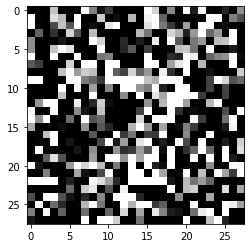
\includegraphics[width=0.5\textwidth]{ErrClass1.png}
    \end{subfigure}
    \begin{subfigure}{0.5\textwidth}
        \centering
        \caption{Target: 0 - Previsto: 5}
        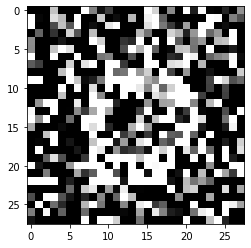
\includegraphics[width=0.5\textwidth]{ErrClass2.png}
    \end{subfigure}
\end{figure}

\begin{figure}[H]
    \begin{subfigure}{0.5\textwidth}
        \centering
        \caption{Target: 6 - Previsto: 5}
        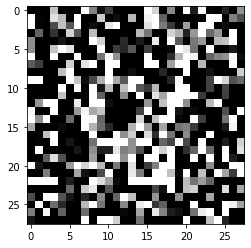
\includegraphics[width=0.5\textwidth]{ErrClass3.png}
    \end{subfigure}
    \begin{subfigure}{0.5\textwidth}
        \centering
        \caption{Target: 1 - Previsto: 2}
        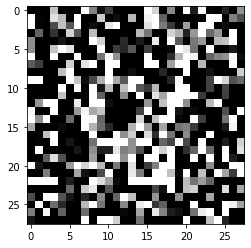
\includegraphics[width=0.5\textwidth]{ErrClass4.png}
    \end{subfigure}
\end{figure}

\begin{figure}[H]
    \centering
    \caption{Target: 1 - Previsto: 5}
    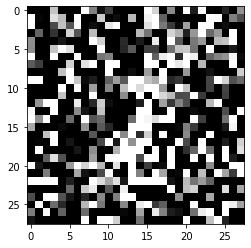
\includegraphics[width=0.25\textwidth]{ErrClass5.png}
\end{figure}

Per quanto riguarda la variante convoluzionale, il risultato risulta essere:
\begin{figure}[H]
    \centering
    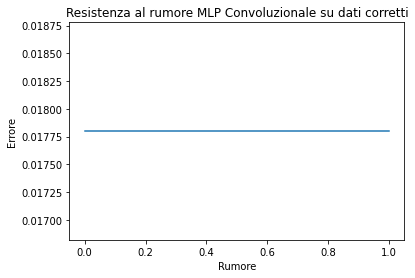
\includegraphics[width=0.50\textwidth]{TPConv.png}
\end{figure}

Sorprendetemente, il livello di accuratezza rimane stabile intorno al \(0.9822\), per cui la rete rimarrà affidabile per tutti i valori di rumore compresi tra \([0.0, 1.0]\).\\
Di seguito alcuni esempi di valori classificati erroneamente:
\begin{figure}[H]
    \begin{subfigure}{0.5\textwidth}
        \centering
        \caption{Target: 3 - Previsto: 9}
        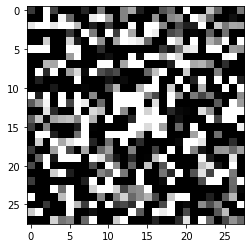
\includegraphics[width=0.5\textwidth]{ErrConv1.png}
    \end{subfigure}
    \begin{subfigure}{0.5\textwidth}
        \centering
        \caption{Target: 0 - Previsto: 3}
        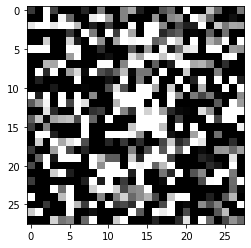
\includegraphics[width=0.5\textwidth]{ErrConv2.png}
    \end{subfigure}
\end{figure}

\begin{figure}[H]
    \begin{subfigure}{0.5\textwidth}
        \centering
        \caption{Target: 1 - Previsto: 2}
        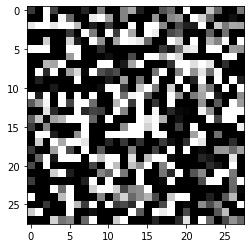
\includegraphics[width=0.5\textwidth]{ErrConv3.png}
    \end{subfigure}
    \begin{subfigure}{0.5\textwidth}
        \centering
        \caption{Target: 0 - Previsto: 2}
        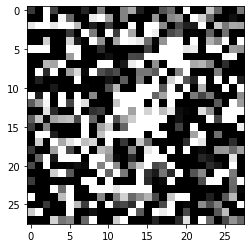
\includegraphics[width=0.5\textwidth]{ErrConv4.png}
    \end{subfigure}
\end{figure}

\begin{figure}[H]
    \centering
    \caption{Target: 8 - Previsto: 9}
    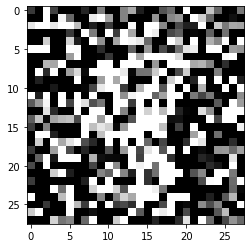
\includegraphics[width=0.25\textwidth]{ErrConv5.png}
\end{figure}

\newpage
\section{Secondo Quesito --- Variazione dell'Accuratezza su Addestramento Rumoroso}
\paragraph{Warning:} Dato che nella sezione saranno definite molte MLP, onde evitare tempi di attesa troppo lunghi, le iterazioni massime sono state ridotte da 15 a 5. La necessità di creare nuove MLP è data dal fatto che il sovrapporsi di addestramenti sulla stessa rete potrebbe influire positivamente sulla predizione e creare di conseguenza dei falsi positivi dato che non si saprà quale degli addestramenti ha massimizzato la resa.
\subsection{Accuratezza su di un Pattern di Test dopo Addestramento Rumoroso}
Prima di tutto, verranno inizializzate 10 MLP, ognuna delle quali sarà addestrata per un singolo e diverso rumore. Di seguito le curve di apprendimento delle reti:
\begin{figure}[H]
    \begin{subfigure}{0.5\textwidth}
        \centering
        \caption{Rumore 0.1}
        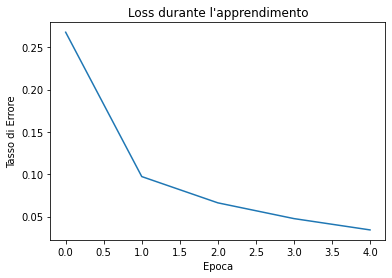
\includegraphics[width=0.80\textwidth]{Rumore1.png}
    \end{subfigure}
    \begin{subfigure}{0.5\textwidth}
        \centering
        \caption{Rumore 0.2}
        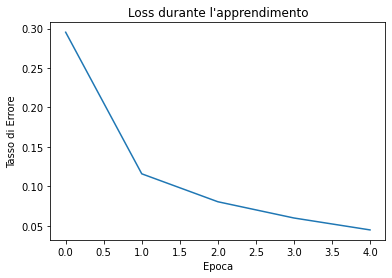
\includegraphics[width=0.80\textwidth]{Rumore2.png}
    \end{subfigure}    
\end{figure}

\begin{figure}[H]
    \begin{subfigure}{0.5\textwidth}
        \centering
        \caption{Rumore 0.3}
        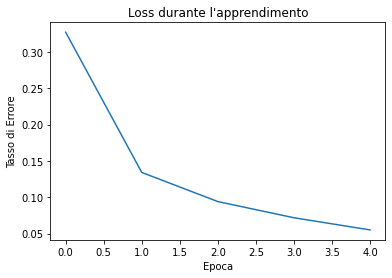
\includegraphics[width=0.80\textwidth]{Rumore3.png}
    \end{subfigure}    
    \begin{subfigure}{0.5\textwidth}
        \centering
        \caption{Rumore 0.4}
        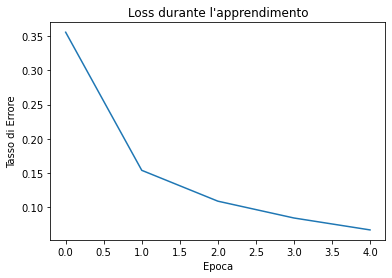
\includegraphics[width=0.80\textwidth]{Rumore4.png}
    \end{subfigure}  
\end{figure}  

\begin{figure}[H]
    \begin{subfigure}{0.5\textwidth}
        \centering
        \caption{Rumore 0.5}
        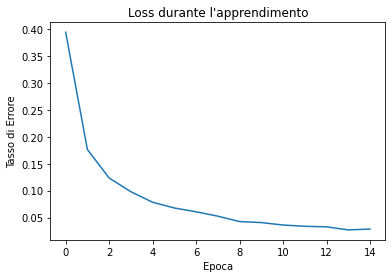
\includegraphics[width=0.80\textwidth]{Rumore5.png}
    \end{subfigure}    
    \begin{subfigure}{0.5\textwidth}
        \centering
        \caption{Rumore 0.6}
        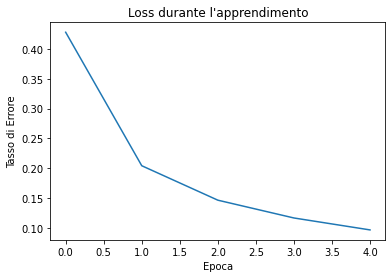
\includegraphics[width=0.80\textwidth]{Rumore6.png}
    \end{subfigure}  
\end{figure}

\begin{figure}[H]
    \begin{subfigure}{0.5\textwidth}
        \centering
        \caption{Rumore 0.7}
        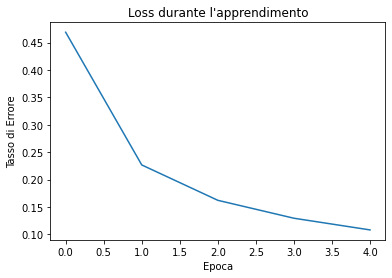
\includegraphics[width=0.80\textwidth]{Rumore7.png}
    \end{subfigure}    
    \begin{subfigure}{0.5\textwidth}
        \centering
        \caption{Rumore 0.8}
        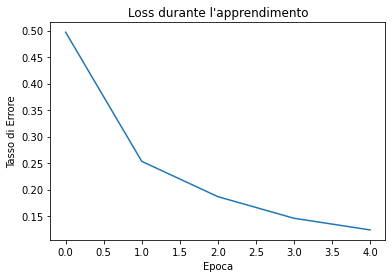
\includegraphics[width=0.80\textwidth]{Rumore8.png}
    \end{subfigure}  
\end{figure}

\begin{figure}[H]
    \begin{subfigure}{0.5\textwidth}
        \centering
        \caption{Rumore 0.9}
        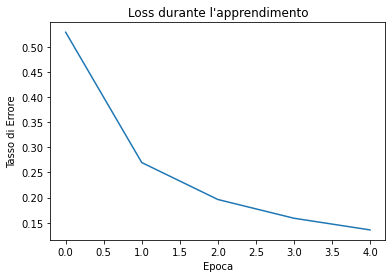
\includegraphics[width=0.80\textwidth]{Rumore9.png}
    \end{subfigure}    
    \begin{subfigure}{0.5\textwidth}
        \centering
        \caption{Rumore 0.10}
        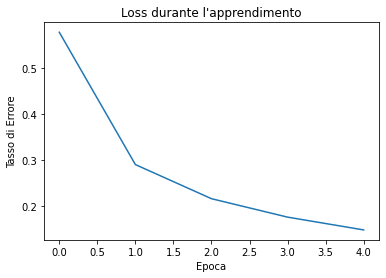
\includegraphics[width=0.80\textwidth]{Rumore10.png}
    \end{subfigure}       
\end{figure} 

\subsection{Definizione di un Valore di Rumorosità Ottimale}
Allo stato attuale, l'accuratezza della MPL classica al variare del rumore risulta:
\begin{itemize}
    \item Rumore 0.1: 0.6258
    \item Rumore 0.2: 0.5855
    \item Rumore 0.3: 0.5847
    \item Rumore 0.4: 0.5826
    \item Rumore 0.5: 0.6005
    \item Rumore 0.6: 0.4644
    \item Rumore 0.7: 0.4529
    \item Rumore 0.8: 0.4305
    \item Rumore 0.9: 0.4958
    \item Rumore 1.0: 0.4208
\end{itemize}

Di conseguenza, i due rumori che massimizzano la resa della rete sono \(0.1\) e \(0.5\).

\newpage
\section{Terzo Quesito --- Variazione dell'Accuratezza su Pattern di Addestramento Ridotto}
\paragraph{Warning: }Dato che i dataset sono estremamente ristretti, si utilizzerà nuovamente un addestramento di 15 cicli.
\paragraph{Warning: }Per mostrare al meglio la variazione dell'accuratezza al diminuire del set di training, si suddividerà il quesito in 3 fasi.\\\\
\\
Prima di tutto, si suddividerà il training set in 3 parti, una da 30.000 elementi, un altra da 15.000 e l'ultima da 6.000. Da notare che crescendo di dimensione, ogni train set contiene anche tutto il set di addestramento della dimensione precedente. \\
Come per il quesito 2, verranno create 3 diverse MLP per evitare che l'addestramento multiplo falsifichi i risultati nel test.
\subsection{50\% del Training Set}
Dopo l'addestramento la curva dell'apprendimento risulta essere
\begin{figure}[H]
    \centering
    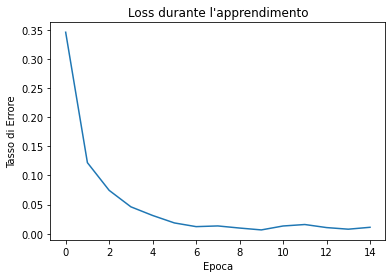
\includegraphics[width=.5\textwidth]{Set50.png}
\end{figure}

Procedendo poi con il test, l'accuratezza si attesta intorno al \(0.9773\) con relativa matrice di confusione:
\begin{figure}[H]
    \centering
    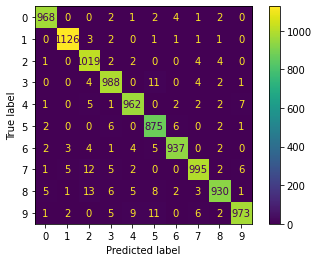
\includegraphics[width=.5\textwidth]{Matrix50.png}
\end{figure}

\subsection{25\% del Training Set}
Dopo l'addestramento la curva dell'apprendimento risulta essere
\begin{figure}[H]
    \centering
    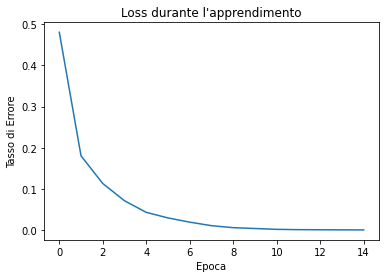
\includegraphics[width=.5\textwidth]{Set25.png}
\end{figure}

Procedendo poi con il test, l'accuratezza si attesta intorno al \(0.9718\) con relativa matrice di confusione:
\begin{figure}[H]
    \centering
    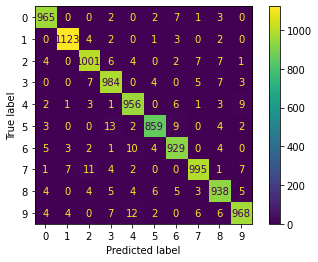
\includegraphics[width=.5\textwidth]{Matrix25.png}
\end{figure}

\subsection{10\% del Training Set}
Dopo l'addestramento la curva dell'apprendimento risulta essere
\begin{figure}[H]
    \centering
    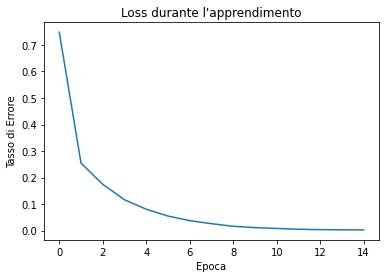
\includegraphics[width=.5\textwidth]{Set10.png}
\end{figure}

Procedendo poi con il test, l'accuratezza si attesta intorno al \(0.9503\) con relativa matrice di confusione:
\begin{figure}[H]
    \centering
    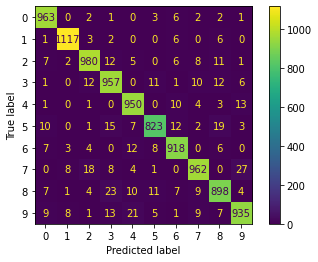
\includegraphics[width=.5\textwidth]{Matrix10.png}
\end{figure}

In conclusione, la riduzione del \textit{training set} riduce di circa \(0.02\) l'accuratezza della rete. Risultato abbastanza sorprendente, in quanto si aumenta l'errore di una piccolissima quantità, ossia un \(2\%\).

\newpage
\section{Conclusioni}
In conclusione, visti gli esiti dei vari quesiti, possiamo affermare che:
\begin{itemize}
    \item Globalmente, le MLP convoluzionali superano per affidabilità le MLP classiche;
    \item Per le MLP classiche, i risultati migliori si ottengono con numero ideale di strati nascosti compreso nell'intervallo \([2, 5]\) e un numero di neuroni nell'intervallo \([250 , 500]\);
    \item Per le MLP convoluzionali, i risultati migliori si ottengono con 5 strati convoluzionali e un numero di filtri e dimensione dei kernel relativamente crescenti;
    \item Sul dataset fornito, per le MLP classiche il numero classificato in modo errato più volte è il numero "8", mentre per le varianti convoluzionali è il "9". Quando si aggiunge rumore, il tasso di errore della variante convoluzionale rimane stabile mentre per la versione classica aumenta esponenzialmente;
    \item I valori di rumore che massimizzano la resa della MLP sono \(0.2\) e \(0.5\);
    \item Anche riducendo drasticamente il \textit{training set}, l'accuratezza rimane stabile al di sopra dello \(0.9\)
\end{itemize}

Ci tengo a segnalare che lo studio non risulta completo, in quanto, per avere dei risultati solidi, bisognerebbe utilizzare molti altri tipi di MLP, con diversi tassi di \textit{learning rate}, diversi risolutori, diversi cicli di addestramento, allenamenti su più rumori e diversi strati convoluzionali.

\end{document}
